\documentclass[ignorenonframetext,hyperref={pdftex,unicode}]{beamer}
%\documentclass[aspectratio=169,ignorenonframetext,hyperref={pdftex,unicode}]{beamer}  %соотношение 16:9

\usepackage{amssymb,amsmath,mathtext} %поддержка формул и русского текста в них
\usepackage{indentfirst,amsfonts} %поддержка русского стиля оформления текста и формул
%\usepackage{makecell,multirow,longtable} %поддержка таблиц занимающих несколько страниц

\usepackage[english,russian]{babel}
\usepackage[T2A]{fontenc}
\usepackage[utf8]{inputenc} %кодировка исходника

% for hyperlinks
\usepackage{hyperref}
% for strike-out text
\usepackage[normalem]{ulem}

\ifpdf
        \usepackage{cmap} % чтобы работал поиск по PDF
        %\usepackage[pdftex]{graphicx}
        \pdfcompresslevel=9 % сжимать PDF
\else
        \usepackage{graphicx}
\fi

\usetheme{Samsolutions} %корпоративная тема

%\setbeamercovered{transparent} %полупрозрачные скрытые элементы

\title{Давайце зробім лінуксоўку больш адкрытай} %название презентации
%\subtitle{SUBTITLE} %подназвание
\author["Андрэй Захарэвіч"]{Андрэй Захарэвіч\\ andrej@zahar.ws} %автор


\begin{document} %начало документа

\frame{\titlepage} % Создание заглавной страницы


\section{Што ужо зроблена} %названия секций для оглавления

\begin{frame}{Што зроблена на дадзены момант} %новый слайд и его название
	\begin{itemize}
		\item \textbf{Анонсы.} \emph{Робяцца некалькімі ўдзельнікамі суполкі}
		\item \textbf{Трамвайны сцэнар.} \emph{Заўжды ёсць запасны варыянт}
		\item \textbf{Мы ў стане зладзіць відэафіксаванне дакладаў}
	\end{itemize}
	\begin{center}
 		
\includegraphics{what_we've_done} %так вставляется картинка
	\end{center}
\end{frame} %конец слайда

\section{Што гераічна праспалі}
\begin{frame}{Ці дастаткова гэтага?} 
	\begin{center}
 		
\includegraphics[height=.8\textheight]{Alwaysdoneit} 
	\end{center}
\end{frame} %конец слайда

\subsection{Анонсы}
\begin{frame}{Анонсы}
	\begin{itemize}
		\item \textbf{Паскарэнне з'яўлення анонсаў}
		\item \textbf{Пашырэнне аўдыторыі?}
	\end{itemize}
	\begin{center}
		
\includegraphics[height=156pt]{survey-announce}
	\end{center}
\end{frame}

\subsection{Справаздачы}
\begin{frame}{Справаздачы}
	\begin{itemize}
		\item \textbf{Справаздачы ў дапаўненне да анонсаў на розных пляцоўках}
		\item \textbf{Апрацоўка адснятага відэаматэрыялу}
		\item \textbf{Рэгулярнае выкладанне слайдаў}
	\end{itemize}
	\begin{center}
		
\includegraphics{Time-to-Share}
	\end{center}
\end{frame}

\subsection{Каардынацыя працы}
\begin{frame}{Спіс задач і каардынацыя}
	\begin{itemize}
		\item \textbf{Публікацыя спіса задач}
		\item \textbf{Магчымасць дадаць задачу}
		\item \textbf{Магчымасць прапісаць сябе адказным за задачу}
	\end{itemize}
	\begin{center}
		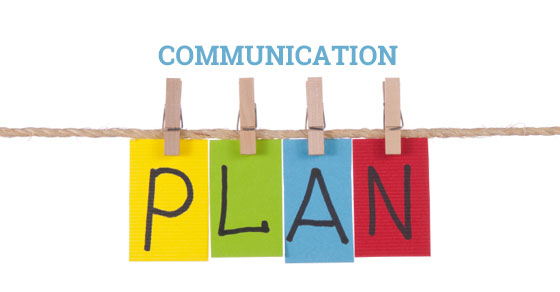
\includegraphics[height=170pt]{communication-plan}
	\end{center}
\end{frame}

\section{Прапановы?}
\frame{\finalslide{Прапановы і пажаданні?}} %слайд вопросы?

\end{document}
